% !TEX root = quickstep.tex

\section{Evaluation} \label{evaluation}
In this section, we present results from an empirical evaluation comparing Quickstep with other systems. We note that performance evaluation is always a tricky proposition as there are a large number of potential systems to compare with. Our goal here is to compare with popular systems that allow running end-to-end queries for TPC-H and SSB benchmarks, and pick three popular representative systems that each have different approaches to high performance analytics, and support stand-alone/single node in-memory query execution. We note that a large number of different SQL data platforms have been built over the past four decades, and a comparison of all systems in this ecosystem is beyond the scope of our study.

%We also note that there are a number of recent systems that address parts of queries in such benchmarks (e.g.~\cite{Vodoo}), but to the best of our knowledge end-to-end

The three open-source systems that we use are MonetDB~\cite{monetdb}, PostgreSQL~\cite{postgres} and Spark~\cite{Spark, SparkSQL} and the commercial system is VectorWise~\cite{vectorwise}. 
We note that there is a lack of open-source in-memory systems that focus on high-performance on a single node (the focus of the Quickstep system). 
VectorWise and Hyper~\cite{hyper} are newer systems, and though informal claims for them easily outperforming MonetDB can often be heard at conferences, that aspect has never been cataloged before. 
We hope that using both VectorWise  and MonetDB in our study fills part of this gap. 
We would have liked to try Hyper, as both VectorWise and Hyper represent systems in this space that were designed over the last decade; but as readers may be aware, Hyper is no longer available for evaluation.
%We also note that the open-source nature of Quickstep means that anyone can use Quickstep for benchmarking without needing to hide the product name, allowing more transparent comparisons across different papers on the same topic. Furthermore, access to the source code allows one to better understand the reasons behind certain performance behaviors, which is otherwise hard to do when only binaries are available.
%(We also point out that there are no recent in-memory database engines that the community can openly experiment with. We hope that with this paper we can help address this issue by presenting an open-source system, which can now allow the research community to actually understand the factors behind end-to-end performance behavior, which often is hard to do when only binaries are available and/or license restrictions prevent disclosing the actual system being used).

Next, we outline our reasons for choosing these systems.
MonetDB, is an early column-store database engine that has seen over two decades of development.
%We use their latest release (December 2016 release and the associated bugfixes).
We also compare with VectorWise, which is a commercial column store system with origins in MonetDB.
%We use the latest release that is available for free evaluation.
PostgreSQL is representative of a traditional relational data platform that has had decades to mature, and is also the basis for popular MPP databases like CitusDB~\cite{citusdata}, GreenPlum~\cite{greenplum}, and Redshift~\cite{redshift}. We use PostgreSQL v.~9.6.2, which includes about a decade's worth of work by the community to add intra-query parallelism~\cite{pg-parallelquery}.
We chose Spark as it is an increasingly popular in-memory data platform. Thus, it is instructive just for comparison purposes, to consider the relative performance of Quickstep with Spark. We use Spark 2.1.0, which includes the recent improvements for vectorized evaluation~\cite{spark-10x-in-2}.

\subsection{Workload} \label{exp-workload}
For the evaluation, we use the TPC-H benchmark at scale factor 100 %(\texttildelow 100GB in size)
as well as the Star Schema Benchmark (SSB) at scale factors 50 and 100. % (\texttildelow 50 GB and 100 GB in size).
Both these benchmarks illustrate workloads for decision support systems.

For the results presented below, we ran each query 5 times in succession in the same session. Thus, the first run of the query fetches the required input data into memory, and the subsequent runs are ``hot.'' We collect these five execution times and report the average of the middle three execution times.

\subsection{System Configuration} \label{exp-system}
For the experiments presented below, we use a server that is provisioned as a dedicated ``bare-metal'' box in a larger cloud infrastructure~\cite{RicciEide:login14}. The server has two Intel Xeon E5-2660 v3 2.60 GHz (Haswell EP) processors. Each processor has 10 cores and 20 hyper-threading hardware threads. The machine runs Ubuntu 14.04.1 LTS. The server has a total of 160GB ECC memory, % (10 x 16 GB DDR4 2133 MHz dual rank RDIMMs),
with 80GB of directly-attached memory per NUMA node. Each processor has a 25MB  L3 cache, which is shared across all the cores on that processor. Each core has a 32KB L1 instruction cache, 32KB L1 data cache, and a 256KB L2 cache.
%This server also has two 1.2 TB 10K RPM SAS HDDs, and one 480 GB SAS SSD device.\reminder{Is disk info necessary?}

%We note that the memory configuration in this sever is not ``balanced'' as there are 5 DIMMS per socket, and each socket has a total of 8 DIMM slots. (Presumably the empty DIMM slots can be used to potentially upgrade the server memory in the future.)

\subsection{System Tuning} \label{exp-tuning}
Tuning systems for optimal performance is a cumbersome task, and much of the task of tuning is automated in Quickstep.
%One of the goals of \Quickstep\ is to operate at high performance without requiring the user to set %any performance ``knobs.''
When \Quickstep\ starts, it automatically senses the available memory and grabs about 80\% of the memory for its buffer pool.
%(There is a command line flag that can be used to explicitly specify the buffer pool size and override this default.)
This buffer pool is used for both caching the database and also for creating temporary data structures such as hash tables for joins and aggregates. \Quickstep\ also automatically determines the maximum available hardware parallelism, and uses that to automatically determine and set the right degree of intra-operator and intra-query parallelism. As noted in Section~\ref{block-structure}, Quickstep allows both row-store and column-store formats. These are currently specified by the users when creating the tables, and we find that for optimal performance, in most cases, the fact tables should be  stored in (compressed) column store format, and the dimension tables in row-store formats. We use this \textit{hybrid} storage format for the databases in the experiments below.

MonetDB too aims to work without performance knobs. MonetDB however does not have a buffer pool, so some care has to be taken to not run with a database that pushes the edge of the memory limit. MonetDB also has a read-only mode for higher performance, and after the database was loaded, we switched to this mode.

The other systems require some tuning to achieve good performance, as we discuss below.

For VectorWise, we increased the buffer pool size to match the size of the memory on the machine (VectorWise has a default setting of 40 GB). We also set the number of cores and the maximum parallelism level flags to match the number of cores with hyper-threading turned on.

%For PostgreSQL we tried both the stable 9.5 version and 9.6 Beta1. The latter has a new feature for intra-operator parallelism that resulted in a 3X higher query performance for the SSB queries. In the results presented below we only show results for Postgres 9.6 Beta1.
PostgreSQL was tuned to set the degree of parallelism to match the number of hyper-threaded cores in the system. In addition, the shared buffer space was increased to allow the system to cache the entire database in memory. The temporary buffer space was set to about half the shared buffer space. % and the worker memory was set to 1GB.
This combination produced the best performance for PostgreSQL. %The TPC-H queries 17 and 20 ran for longer than an hour on PostgreSQL, and we aborted these queries.

Spark was configured in standalone mode and queries were issued using Spark-SQL from a Scala program. %, submitted to Spark using \texttt{spark-submit}.
We set the number of partitions (\texttt{spark.sql.shuffle.partitions}) to the number of hyperthreaded cores. We experimented with various settings for the number of workers and partitions, and used the best combination. This combination was often when the number of workers was a small number like 2 or 4 and the number of partitions was set to the number of hyper-threaded cores. %We found the best results with 4 workers, and 40 partitions.

Unlike the other systems, Spark sometimes picks execution plans that are quite expensive. For example, for the most complex queries in the SSB benchmark (the Q4.X queries), Spark choses a Cartesian product. As a result, these queries crashed the process when it ran out of memory. We rewrote the \texttt{FROM} clause in these queries to enforce a better join order. We report results from these rewritten queries below.

\begin{figure*}
	\center
	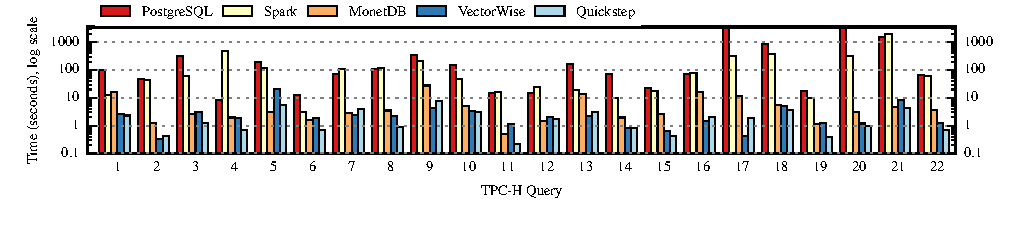
\includegraphics[]{system/figures/all-tpch-sf100.pdf}
	\caption{\textbf{Comparison with TPC-H, scale factor 100. Q17 and Q20 did not finish on PostgreSQL after an hour.}} %, and were aborted.}
	\label{fig-tpch-sf100}
\end{figure*}


\subsection{TPC-H at Scale Factor 100} \label{exp-tpch-sf-100}

Figure~\ref{fig-tpch-sf100} shows the results for all systems when using the TPC-H dataset at SF 100 (\texttildelow 100GB dataset).

As can be seen in Figure~\ref{fig-tpch-sf100}, Quickstep far outperforms MonetDB, PostgreSQL and Spark across all the queries, and in many cases by an order-of-magnitude (the y-axis is on a log scale). These gains are due to three key aspects of the design of the Quickstep system: the storage and scheduling model that maximally utilize available hardware parallelism, the template metaprogramming framework that ensures that individual operator kernels run efficiently on the underlying hardware, and the query processing and optimization techniques that eliminate redundant work using cache-efficient data structures. Comparing the total execution time across all the queries in the benchmark, both Quickstep and VectorWise are about \textbf{2X} faster than MonetDB and \textbf{orders-of-magnitude} faster than Spark and PostgreSQL.

When comparing Quickstep and VectorWise, the total run times for the two systems (across all the queries) is 46s and 70s respectively, making Quickstep $\sim$34\% faster than VectorWise. Across each query, there are queries where each system outperforms the other. Given the closed-source nature of VectorWise, we can only speculate about possible reasons for performance differences.

VectorWise is significantly faster (at least 50\% speedup) in 3 of the 22 queries. The most common reason for Quickstep's slowdown is the large cost incurred in materializing intermediate results in queries with deep join trees, particularly query 7. While the use of partial push-down greatly reduced this materialization cost already (by about 6X in query 7, for instance), such queries produce large intermediate results. Quickstep currently does not have an implementation for late materialization of columns in join results~\cite{Shrinivas2013Materialization}, which hurts its performance. Quickstep also lacks a fast implementation for joins when the join condition contains non-equality predicates (resulting in 4X slowdown in query 17), as well as for aggregation hash tables with composite, variable-length keys (such as query 10).

On the other hand, Quickstep significantly outperforms VectorWise (at least 50\% speedup) in 10 of the 22 queries. Across the board, the use of LIP and exact filters improves Quickstep's performance by about 2X. In particular, Quickstep's 4X speedup over VectorWise in query 5 can be attributed to LIP (due to its deep join trees with highly selective predicates on build-side). Similarly, we attribute a speedup of 4.5X in query 11 to exact filters, since every one of the four hash joins in a naive query plan is eliminated using this technique. The combination of these features also explains about 2X speedups in queries 3 and 11. We also see a 4.5X speedup for query 6, which we have not been able to explain given that we only have access to the VectorWise binaries. Query 19 is 3X faster in Quickstep. This query benefits significantly from the partial predicate push-down technique  (cf. Section~\ref{sec-pushdown-disj-preds}). VectorWise appears to also do predicate pushdown~\cite{BonczNE13}, but its approach may not be as general as our approach.

For the remaining 9 queries, Quickstep and VectorWise have comparable running times.
We have also carried out similar experiments using the SSB benchmark; these results are reported in~\cite{patel1quickstep}.

As noted above (cf. Section~\ref{exp-tuning}), Quickstep uses a hybrid database format with the fact table is stored in compressed column store format and the dimension tables in a row store format. For the TPC-H SF 100 dataset, we ran an experiment using a pure row store and pure compressed column store format for the \textit{entire} database. The hybrid combination was 40\% faster than the pure compressed column store case, and 3X faster than the pure row store case, illustrating the benefit of using a hybrid storage combination. We note that these results show smaller improvements for column stores over row stores compared to earlier comparisions, e.g.~\cite{DBLP:conf/sigmod/AbadiMH08}; although this previous work has used indirect comparisons using the SSB benchmark and across two different systems.

\subsection{Denormalizing for higher performance}
\label{denormalizing}
In this experiment, we consider a technique that is sometimes used to speed up read-mostly data warehouses. The technique is denormalization, and data warehousing software product manuals often recommend considering this technique for read-mostly databases (e.g.~\cite{denorm-SQL, denorm-IBM, denorm-sybase}).

For this experiment, we use a specific schema-based denormalization technique that has been previously proposed~\cite{widetable}. This technique walks through the schema graph of the database, and converts all foreign-key primary-key ``links'' into an outer-join expression (to preserve NULL semantics). The resulting ``flattened'' table is called a WideTable, and it is essentially a denormalized view of the entire database. The columns in this WideTable are stored as column stores, and complex queries then become scans on this table.

An advantage of the WideTable-based denormalization is that it is largely agnostic to the workload characteristics (it is a schema-based transformation). Thus, it is easier to use in practice than selected materialized view methods.

\begin{figure*}
	\center
	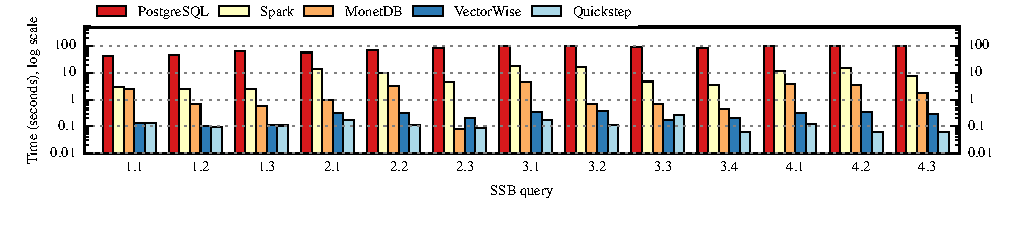
\includegraphics[]{system/figures/all-ssb-wt50.pdf}
	\caption{\textbf{Comparison with denormalized SSB, scale factor 50.}}
	\label{fig-ssb-sf50-widetable}
	%\vspace*{-1em}
\end{figure*}

We note that every denormalization technique has the drawback of making updates and data loading more expensive. For example, loading the denormalized WideTable in \Quickstep\ takes about 10X longer than loading the corresponding normalized database. Thus, this method is well-suited for very low update and/or append only environments.

For this experiment, we used the SSB dataset at scale factor 50. The raw denormalized dataset file is 128GB.

The results for this experiment are shown in Figure~\ref{fig-ssb-sf50-widetable}. The total time to run all thirteen queries is 1.6s, 3.2s, 	23.2s, 1,014s, and	111.9s across Quickstep, VectorWise, MonetDB, PostgreSQL and Spark respectively. Quickstep's  advantage over MonetDB now increases to over an order-of-magnitude (\textbf{14X}) across most queries.
%Curiously, if we compare Figures~\ref{fig-ssb-sf50-detail} and~\ref{fig-ssb-sf50-widetable} we noticed that \Quickstep\ benefits from the denormalization technique by a factor of about 5X. However, MonetDB actually gets a little slower.
MonetDB struggles with the WideTable that has 58 attributes. MonetDB uses a BAT file format, in which it stores the pair (attribute and object-id) for each column. In contrast, \Quickstep's block-based storage design does not have the overhead of storing the object-id/tuple-id for each attribute (and for each tuple). The disk footprint of the database file is only 42 GB for \Quickstep\ while it is 99 GB for MonetDB. Tables with such large schemas hurt MonetDB, while \Quickstep's storage design allows it to easily deal with such schemas. Since queries now do not require joins (they become scans on the WideTable), \Quickstep\ sees a significant increase in performance.
\Quickstep\ is also about \textbf{2X} faster than VectorWise, likely because of similar reasons as that for MonetDB. To the best of our knowledge, the internal details about VectorWise's implementation have not been described publicly, but they likely inherit aspects of MonetDB's design, since the database disk footprint is 63 GB.

\twoabfigures
{system/figures/ssb-sf100-storage-format-comparison-total}
{system/figures/ssb-sf100-storage-format-comparison}
{\textbf{Impact of storage format on performance for SSB scale factor 100\vspace*{3em}}}
{fig-ssb-sf100-rowstore}
{Overall speedup}
{Detailed query speedups}
{bht}

\Quickstep's speedup over the other systems also continues when working with tables with a large number of attributes. Compared to Spark and PostgreSQL, \Quickstep\ is \textbf{70X} and \textbf{640X} faster. Notice that compared to the other systems, PostgreSQL has only a pure row-store implementation, which hurts it significantly when working with tables with a large number of attributes.

\subsection{Impact of Row Store vs. Column Store}
\label{sec:expt:rs-vs-cs}

As described in Section~\ref{storage-manager}, \Quickstep\ supports both row store and column store formats. %By default all tables are stored in a column store format. However, tables can be created in either format, which allows for an easy comparison of different storage formats (and potentially allows for investigating new storage formats).
In this experiment, we use the multiple storage format feature in Quickstep to study the impact of different storage layouts, and specifically we compare a row-store versus a column-store layout. A notable example of such comparison is the work by Abadi et al.~\cite{DBLP:conf/sigmod/AbadiMH08}, in which the SSB benchmark was used to study this aspect, but across two \textit{different} systems -- one that was a row-store system and the other was a column-store (C-store)~\cite{StonebrakerABCCFLLMOORTZ05}.  In this experiment, we also use the SSB benchmark, but we use a 100 scale factor dataset (instead of the 10 scale factor datase that was used in~\cite{DBLP:conf/sigmod/AbadiMH08}).

In Figure~\ref{fig-ssb-sf100-rowstore}, we show the speedup of the (default) column store compared to the row store format.
The use of a column store format leads, unsurprisingly, to higher performance over using a row store format. %The total time to run the benchmark improves by about 2X as shown in Figure~\ref{fig-ssb-sf100-rowstore} (a).
The simpler Q1.Y queries show far bigger improvements as the input table scan is a bigger proportion of the query execution time. The other queries spend a larger fraction of their time on joins, and passing tuples between the join operations. Consequently, switching to a column store has a less dramatic improvement in performance for these queries.

An interesting note is that the impact of column stores here is  smaller than previous comparisons~\cite{DBLP:conf/sigmod/AbadiMH08} which have compared these approaches across two different systems and showed about a 6X improvement for column-stores. Overall, we see a 2X improvement for column-stores, which is lower than these previous results.
One key reason for the lower improvement is because column stores typically help speed up scans (select operators).
However query plans are often complex with several different types of operators. 
Thus while considering overall query execution time, selection forms one fraction of the overall time distribution. 

We have also experimented with compressed column-stores in this same setting, and find that they are slower than non-compressed column stores. Compressed column stores are still faster than row store by about 50\% overall. But compression adds run-time CPU overhead which reduces is overall performance compared to regular column stores. 
The results for TPC-H are similar. 
We present the TPC-H results in Chapter~\ref{chap:pipeline}, where we also discuss the impact of various dimensions like storage format, parallelism and block size on the performance of pipelined query processing.

%We note that the end-to-end impact of a Column Store for entire queries is in some cases quite small. Within \Quickstep\ pipelines, the impact of columnstores is quite small. That is, operations like HashJoin or Sort are not effected as severely by the choice of block type as are simple scans. Thus in queries where simple scans are essentially the only operator, we see huge performance improvements from using columnstores. This is case in the first three queries of SSB where either there are no joins, or the join is eliminated by an optimization. Here columnstores perform nearly three times better than rowstores.


%\subsection{Impact of \Quickstep\ Techniques}
%\label{sec:quickstep-impact}
%In the next set of experiments, we aim to examine the impact of selected individual techniques in \Quickstep\ to determine their individual contribution. With these set of experiments, we leverage the fact that there are multiple implementations in Quickstep and we can use that to carry out a comparison of popular techniques and compare that on contemporary settings. For all the experiments presented in this section, we use SSB SF 100 and the 160 GB server machine that is described in Section~\ref{sec:ssb100}.

\subsection{Template Metaprogramming Impact}
\label{sec:expt:vectorization}

\twoabfigures
{system/figures/copy-elision-comparison-total}
{system/figures/copy-elision-comparison}
{\textbf{Impact of template metaprogramming.}}
{fig-template-metaprogramming}
{Change in total time.}
{Change in the detailed query execution times.}
{bht}

Next, we toggle the use of the template metaprogramming (see Section~\ref{ssec:expression-eval}), using the SSB 100 scale factor dataset. Specifically, we change the compile time flag that determines whether the \texttt{ValueAccessor} is constructed by copying attributes (Basic) or by providing an indirection (Selection). The results for this experiment are shown in Figure~\ref{fig-template-metaprogramming}.

The overall performance impact of eliminating the copy during predicate evaluation is about 20\%. As with the previous experiment, the benefits are larger for the simpler Q1.X queries and lower for the other queries that tend to spend most of their time on join operations and in the pipelines in passing tuples between different join operations.

The result for this experiment with TPC-H show far smaller improvements (see Figure~\ref{fig:tpch-q10-waterfall} for a typical example), as the TPC-H queries spend a far smaller fraction on their overall time on expression evaluation (compared to the SSB queries).

\subsection{Impact of Optimization Techniques}
\label{sec:expt:optimization}

\begin{figure}[t]
	\centering 
	\begin{subfigure}[ht]{0.2\textwidth}
		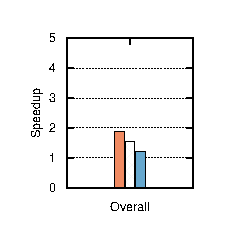
\includegraphics[width=\textwidth]{system/figures/lip-ef-impact-total}
		\caption{Overall}
	\end{subfigure}
	~
	\begin{subfigure}[ht]{0.7\textwidth}
		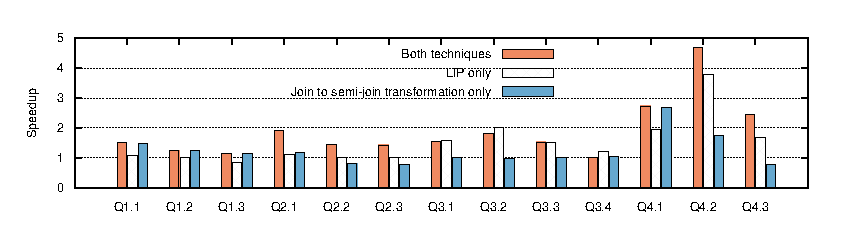
\includegraphics[width=\textwidth]{system/figures/lip-ef-impact}
		\caption{Breakdown of speedup due to techniques}
	\end{subfigure}
	\caption{\textbf{Impact of Exact Filter and LIP using SSB at scale factor 100.}}
	\label{fig-lip-ef-impact}
\end{figure}

We described the novel optimization techniques in \Quickstep\ optimizer in Section~\ref{sec:query-opt}. In this experiment,
we measure the impact of these techniques individually, viz. LIP and join to semi-join transformation.

As with the previous two sections, we use the SSB 100 scale factor dataset. (The results for the TPC-H dataset is similar.)
Figure~\ref{fig-lip-ef-impact} shows the impact of these techniques over a baseline in which neither of these techniques are used. As shown in Figure~\ref{fig-lip-ef-impact}, these techniques together provide a nearly 2X speedup for the entire benchmark. The LIP and semi-join transformation techniques individually provide about 50\% and 20\% speedup
respectively. While some queries do see a slowdown due to the individual techniques, the application of both
techniques together always gives some speedup. In fact, of the 13 queries in the benchmark,
8 queries see at least a 50\% speedup and three queries see at least 2X speedup. The largest speedups
are in the most complex queries (group 4), where we see an overall speedup of more than 3X.

These results validate the usefulness of these techniques on typical workloads. Further, their simplicity of implementation and general applicability leads us to believe that these techniques should be more widely used in other database systems.

\subsection{Elasticity} \label{sec:expt:elasticity}

\begin{figure*}
	\vspace*{3em}
	\centering
	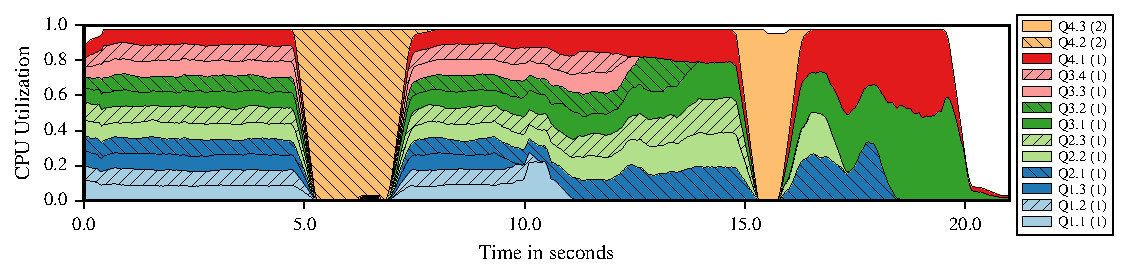
\includegraphics[width=\textwidth]{system/figures/2-high-priority-queries.pdf}
	\caption{\textbf{Prioritized query execution. QX.Y(1) indicates that Query X.Y has a priority 1. Q4.2 and Q4.3 have higher priority (2) than the other queries (1).}}
	\label{fig-high-priority}
\end{figure*}

In this experiment, we evaluate \Quickstep's ability to quickly change the degree of inter-query parallelism, driven by the design of its work-order based scheduling approach (cf. Section~\ref{scheduler}). For this experiment, we use the 100 scale factor SSB dataset. The experiment starts by concurrently issuing the first 11 queries from the SSB benchmark (i.e. Q1.1 to Q4.1), against an instance of Quickstep that has just been spun up (i.e. it has an empty/cold database buffer pool).
All these queries are tagged with equal priority, so the Quickstep scheduler aims to provide an equal share of the resources to each of these queries. While the concurrent execution of these 11 queries is in progress, two high priority queries enter the system at two different time points. The results for this experiment are shown in Figure~\ref{fig-high-priority}.
In this figure, the y-axis shows the fraction of CPU resources that are used by each query, which is measured as the fraction of the overall CPU cycles utilized by the query.

Notice in Figure~\ref{fig-high-priority}, at around the 5 second mark when the high priority query Q4.2 arrives, the \Quickstep\ scheduler quickly stops scheduling work orders from the lower priority queries and allocates all the CPU resources to the high-priority query Q4.2.
As the execution of Q4.2 completes, other queries simply resume their execution.
%\reminder{We might want to increase some font sizes in this figure. Also, pick a color other than red for Q4.1.}

Another high priority query (Q4.3) enters the system at around 15 seconds.
Once again, the scheduler dedicates all the CPU resources to Q4.3 and pauses the lower priority queries.
At around 17 seconds, as the execution of query Q4.3 completes, the scheduler resumes the scheduling of work orders from all remaining active lower priority queries.

\begin{figure}
	\centering
	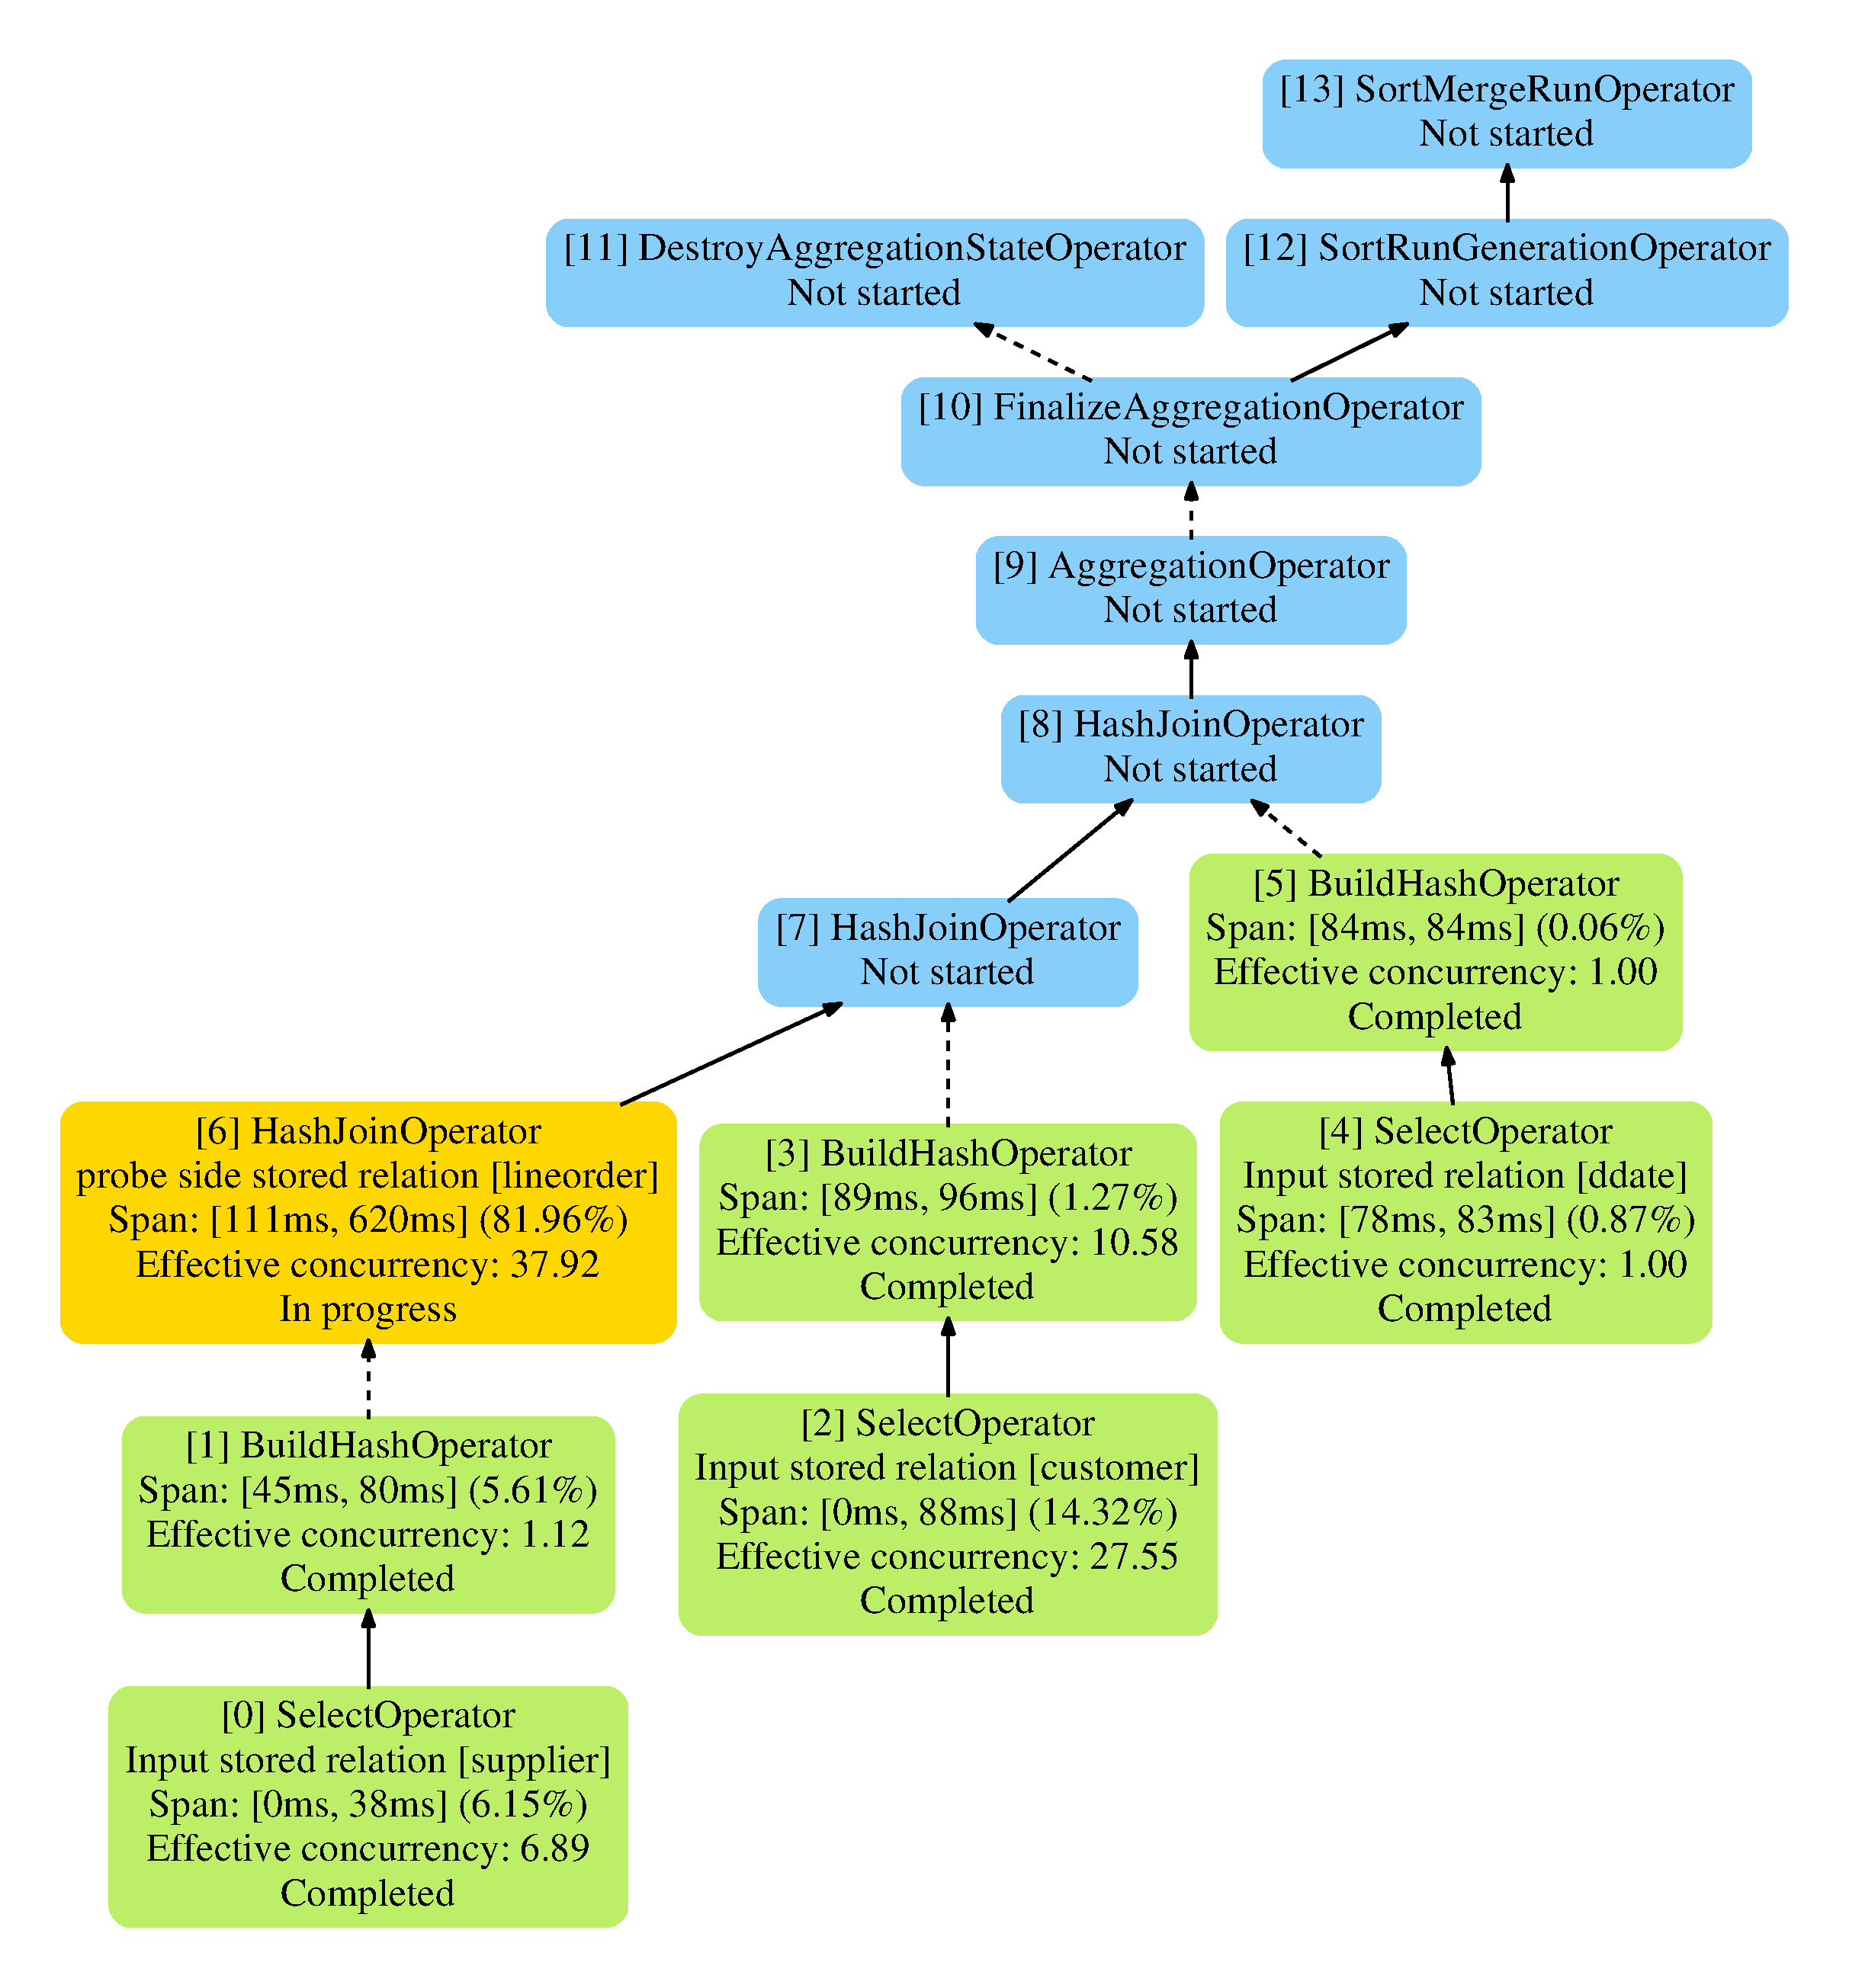
\includegraphics[width=0.6\columnwidth,height=4.2in]{system/figures/q31-progress.pdf}
	\caption{\small \textbf{Query progress status. Green nodes (0-5) indicate work that is completed, the yellow node (6) corresponds to operators whose work-orders are currently being executed, and the blue nodes (7-13) show the work that has yet to be started.}}
	\label{fig-query-progress}
\end{figure}

This experiment highlights two important features of the \Quickstep\ scheduler.
First, it can dynamically and quickly adapt its scheduling strategies. % in favor of the queries with higher priorities.
Second, the \Quickstep\ scheduler can naturally support query suspension (without requiring complex operator code such as~\cite{DavisonG94}), which is an important concern for managing resources in actual deployments.

\subsection{Built-in Query Progress Monitoring}\label{sec:progress-monitoring}
An interesting aspect of using a work-order based scheduler (described in Section~\ref{scheduler}) is that the state of the scheduler can easily be used to monitor the status of a query, without requiring any changes to the operator code. Thus, there is a generic in-built mechanism to monitor the progress of queries.

\Quickstep\ can output the progress of the query as viewed by the scheduler, and this information can be visualized. As an example, Figure~\ref{fig-query-progress} shows the progress of a query with three join operations, one aggregation, and one sort operation.

